\subsection{Overview}

Within a FLAME simulation, every agent only interacts with its environment via the reading and writing of messages to a collection of Message Boards. This makes the Message Board component the ideal candidate for enabling parallelism. With a distributable Message Boards, agents can be farmed out across multiple processing nodes and simulated in parallel, while a coherent simulation can be maintained through the unified view of the distributed Boards.

\begin{figure}[h]
 \centering
  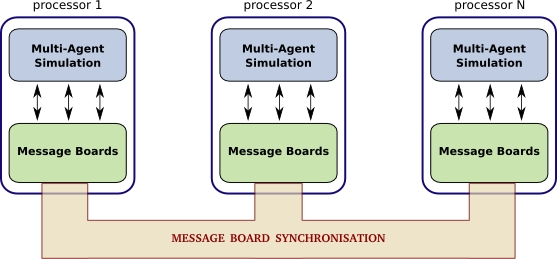
\includegraphics[scale=0.50]{mboard_flame.jpg}
 \caption{Parallelisation of FLAME using distributed Message Boards}
 \label{fig:mb_flame}
\end{figure}

In the recent code release, the Message Board was decoupled from the FLAME framework and implemented as a separate library. This will provides us with the flexibility to experiment with different parallelisation strategies while minimising the impact on current users of the FLAME framework.

The Message Board Library (\textit{libmboard}) was designed as a static library that can be linked to the simulation binaries and accessed via the libmboard Application Program Interface (API). 

\textit{libmboard} uses MPI to communicate between processors, and POSIX threads (pthreads) to fork a separate thread for handling data management and inter-process communication. The use of threads enables the memory intensive operations of managing the Message Boards to be performed concurrently with the agent simulations. 

Apart from potentially making better use of multi-core processors, delegating \textit{libmboard} operations to a separate thread also allows us to minimise the overheads by overlapping the Board synchronisation time with useful computation.